\chapter{動画予測}

  \section{動画予測の定義と定式化}

    動画予測は、既知のビデオフレームの系列から未来のフレームを予測するタスクであり、教師なし学習、または自己教師あり学習の一種として位置付けられる。
    このタスクは、時空間的な連続性と一貫性を持つ未来のフレームシーケンスを生成することを目指す。

    \subsection{動画予測モデル}
    動画予測の目的は、与えられた過去のフレームシーケンスから未来のフレームを予測するモデル \( M \) を最適化することである。
    ほとんどの動画予測モデルにおいて、モデルの扱うシークエンスは入力長と出力長の二つに分割される。入力長は、モデルが予測を行うために必要な過去のフレームであり、一貫してモデルがその動画の時空間的ダイナミクスを学習するために使用される。出力長は、モデルが予測を行う未来のフレームであり、モデルが最終的に生成するフレームシーケンスの一部となり、この部分に対して損失が計算される。また、もっとも初めの出力フレーム以降のフレームでは、直前の出力フレームが入力フレームとして扱われる。
    動画予測モデル \( M \) は、出力長として位置付けられるある時間ステップ\( t\) のフレーム\( \hat{X}_{t} \) を生成する際は、その直前までの過去のフレーム \( X_{0:t-1} \) を入力として受け取り、それに基づいてそれに続く未来のフレームを生成する。
    このプロセスは以下のように定式化される:

    \begin{equation}
    \hat{X}_{t} = M(X_{0:t-1})
    \end{equation}

    \subsection{最適化}
    最適化プロセスは、一連の学習データセットを用いて、損失関数Lを最小化するように動画予測モデル\( M \) のパラメータを調整する。
    このプロセスは、以下のように表現される:

    \begin{equation}
    M_{\text{optimized}} = argmin_{M} L(\hat{X}, X)
    \end{equation}

    ここで、\( M_{\text{optimized}} \) は最適化された予測モデルを表す。

    この損失関数は、予測された未来のフレームと実際の未来のフレームとの差異を測定するために使用され、一般的には平均二乗誤差(Mean Squared Error, MSE)が用いられる。これは、予測されたフレームと実際のフレームのピクセル単位の差異を測定する。MSEは次のように定義される:

    \begin{equation}
    MSE = \frac{1}{N} \sum_{i=1}^{N} (X_i - \hat{X}_i)^2
    \end{equation}

  \section{動画予測のための基礎技術}
    動画予測には、複数のフレーム間での時空間的な関連を捉え、未来のフレームを予測する能力が必要である。この目的を達成するためには、畳み込みニューラルネットワーク(CNN)、エンコーダ・デコーダ構造、長短期記憶(LSTM)、そしてアテンションメカニズムといった複数の技術が組み合わされる。ここではそういった基礎技術群について説明する。

    \subsection{Convolutional Neural Network (CNN)}
      動画予測において、CNNは各フレームの空間的な特徴を抽出する役割を担う。
      動画は時間的な次元を持つ一連の画像であり、各フレームにおける空間的な特徴を理解することは、時間的な次元を解析する前の重要なステップである。

      畳み込みニューラルネットワーク(CNN)は、特に画像認識や動画処理において広く用いられる深層学習の一形態である。
      CNNは、画像の局所的な特徴を捉えるために、畳み込み層とプーリング層を交互に繰り返すことで構成される。
      畳み込み層は画像から特徴を抽出するためのフィルターの役割を果たし、プーリング層は画像の特徴を圧縮する役割を持つ。
      CNNを用いた多くの画像処理アプリケーションにおいては、この畳み込み操作とプーリング操作が連続的に繰り返されることで、入力データの高次元な特徴を抽出することを可能にしている。
      ここでは、その二つの重要な操作について説明する。
    
      \subsubsection{畳み込み}
        CNNの主な特徴は、局所的な特徴を効率的に捉えることができる畳み込み層にある。
        この畳み込み層は、入力された画像から特定の特徴を抽出するフィルターの役割を果たし、これにより画像の特徴を圧縮して表現することができる。
        
        CNNおける畳み込み処理は、入力データに対する特定のカーネルの適用として理解される。カーネルは小規模な行列であり、入力データの局所的な領域に対して適用される。
        この畳み込み操作は、入力データを I、カーネルを K とした場合、以下の式で表される。

        \begin{equation}
          S(i, j) = (I * K)(i, j) = \sum_{m}\sum_{n}I(i+m, j+n)K(m, n)
        \end{equation}

        この操作は、入力データの全域にわたって繰り返され、最終的に特徴マップと呼ばれる新しい行列が生成される。特徴マップには、その入力データにおける特定のパターンや構造が抽出されている。
      
      \subsubsection{プーリング}
        この層の主な目的は、特徴マップの次元を減少させることである。
        具体的には、プーリング層は特徴マップの小さな領域を集約し、その領域内の代表的な値(最大値や平均値)を抽出する。
        この操作により、ネットワークは画像の局所的な変化に対してより頑健になり、より抽象的な特徴表現を学習することが可能である。

        \begin{itemize}
        \item \textbf{最大値プーリング(Max Pooling)}:この手法では、各領域の最大値が選択される。
        これにより、特徴マップから最も強い信号を保持し、関連性の低い信号を破棄する。
        最大値プーリングは、特に画像内のテクスチャや形状などの顕著な特徴を強調するのに有効である。
        ここで、入力となる特徴マップをF, プーリング領域のサイズをm*n, プーリング層の出力をPとすると、最大値プーリングは以下の式で表される。

        \begin{equation}
          P(i, j) = \max_{m}\max_{n}F(i+m, j+n)
        \end{equation}

        \item \textbf{平均値プーリング(Average Pooling)}:平均プーリングは、各領域の平均値を計算する。
        これにより、特徴マップの全体的な特性をより平滑化し、より均一な特徴表現を提供することが可能である。
        ここで、入力となる特徴マップをF, プーリング層の出力をPとすると、平均値プーリングは以下の式で表される。

        \begin{equation}
          P(i, j) = \frac{1}{mn}\sum_{m}\sum_{n}F(i+m, j+n)
        \end{equation}
        
        \end{itemize}

    \subsection{Encoder-Decoder}
      エンコーダ・デコーダ構造は画像処理においても広く用いられ、特にU-Netのようなアーキテクチャが代表的である。
      エンコーダ・デコーダ構造は、一連の入力データを処理し、それを内部表現に変換するエンコーダ部分と、この内部表現から出力を生成するデコーダ部分の二つの主要なコンポーネントから構成される。
      動画予測において入力データとなるのは、動画の各フレームであり、出力データはそれに続く未来のフレームである。
      ここでは画像処理におけるエンコーダ・デコーダ構造に焦点を当てて説明する。
        
      \subsubsection{エンコーダ}
        エンコーダは入力データをCNNによって処理し、それを高次元から低次元の表現に変換する。
        このプロセスは、入力データに含まれる重要な情報を抽出し、より扱いやすいサイズまたは形式に圧縮することを目的とする。
        動画予測アプリケーションにおいては、空間的特徴に加え、複雑な時間的特徴の依存性をモデリングするため、一般的な画像処理ディープラーニングモデルと比較して大量の計算資源を必要とする。
        そのため、エンコーダにより特徴を圧縮し、より低い次元で高度な特徴を抽出することは、計算コストの削減という点からも非常に重要である。
        
      \subsubsection{デコーダ}
        デコーダは本質的にエンコーダの逆処理である。動画予測においては、その直前のアーキテクチャにより生成された内部表現を受け取り、目的とする出力を生成する役割を持つ。
        動画予測の再帰ネットワーク内では、エンコーダにより圧縮された行列が扱われるため、そのままでは出力には不適切である。デコーダはそのような圧縮された表現を元の次元に展開し、出力に適した形式に変換する。

    
    \subsection{Long Short Term Memory (LSTM)}
    

    リカレントニューラルネットワーク(RNN)は、時系列データや自然言語などのシーケンシャルな情報を扱うために開発されたニューラルネットワークの一種である。RNNの特徴は、過去の情報を隠れ状態として保持し、それを利用して次の出力を生成する点にある。しかし、RNNは長期的な依存関係を捉えることに困難を抱えていた。この問題は「勾配消失問題」として知られ、ネットワークが深くなるほど、またはシーケンスが長くなるほど顕著になる。勾配消失問題により、RNNは過去の情報を長期間保持し活用することが困難になる。
    
    この問題を解決するために開発されたのが、長短期記憶(LSTM)である。LSTMは、RNNの基本的な枠組みを保ちつつ、特定の情報を長期間記憶する能力を強化した。LSTMの主要な特徴は、セル状態と呼ばれる内部メカニズムであり、これにより長期的な情報を保持することが可能となる。
    
    LSTMのユニークな構造は以下の三つのゲートから成る:忘却ゲート、入力ゲート、出力ゲート。
    
    1. \textbf{忘却ゲート(Forget Gate)}:このゲートは、セル状態に含まれる情報の一部を削除する役割を担う。LSTMネットワークが長期的な依存関係を学習する過程で、関連性の低い古い情報を捨てることが重要である。忘却ゲートはシグモイド関数を使用して、どの情報を保持し、どの情報を忘れるかを決定する。
   
    2. \textbf{入力ゲート(Input Gate)}:入力ゲートは、新しい情報をどの程度セル状態に追加するかを決定する。このゲートでは、シグモイド関数がどの情報を更新するかを決定し、tanh関数が新しい候補値を生成する。そして、これら二つの値の積が新しい情報としてセル状態に追加される。
    
    3. \textbf{出力ゲート(Output Gate)}:出力ゲートは、現在のセル状態に基づいて、ネットワークの出力を決定する。このゲートは、シグモイド関数を使用して、セル状態のどの部分が出力されるべきかを決定し、tanh関数によって処理されたセル状態との積が最終的な出力となる。
    
    LSTMユニットの数学的な定式化は以下の通りである。\( h_t \) は時刻 \( t \) での隠れ状態、\( c_t \) はセル状態、\( x_t \) は入力、\( f_t \)、\( i_t \)、\( o_t \) はそれぞれ忘却ゲート、入力ゲート、出力ゲートの活性化関数を表す。
    
    \begin{align}
      f_t &= \sigma(W_f \cdot [h_{t-1}, x_t] + b_f) \\
      i_t &= \sigma(W_i \cdot [h_{t-1}, x_t] + b_i) \\
      \tilde{c}_t &= \tanh(W_c \cdot [h_{t-1}, x_t] + b_c) \\
      c_t &= f_t * c_{t-1} + i_t * \tilde{c}_t \\
      o_t &= \sigma(W_o \cdot [h_{t-1}, x_t] + b_o) \\
      h_t &= o_t * \tanh(c_t)
    \end{align}
    
    ここで、\( W \) と \( b \) はそれぞれ重みとバイアスを表し、\( \sigma \) はシグモイド活性化関数、\( \tanh \) は双曲線正接活性化関数を指す。LSTMのこの構造により、長期的な依存関係を効果的にモデル化することが可能となり、特に時系列データや動画予測などの分野において有効である。
    
    \subsection{Attention}

    アテンションメカニズムは、1990年代に自然言語処理(NLP)分野で初めて提案されたが、その真価が広く認識されるようになったのは2014年の「Neural Machine Translation by Jointly Learning to Align and Translate」という論文での再発見以降である。この技術は、モデルが重要な情報に焦点を当て、それ以外の情報を無視する能力を提供することにより、ディープラーニングにおける重要な進歩の一つとなった。

    アテンションメカニズムの中心には、クエリ(Query)、キー(Key)、バリュー(Value)の三つの概念がある。これらの要素を使用して、モデルがどの情報に注意を払うべきかを決定する。

    \begin{itemize}
      \item \textbf{クエリ(Query)}:クエリは現在注目している要素や状態を表し、モデルがどの情報に注目するかを決定する基準となる。
      \item \textbf{キー(Key)}:キーはデータセット内の各要素に関連付けられ、クエリとの関係を定義する。クエリとキーの間の類似性が高いほど、そのキーに関連付けられた情報に注意が向けられる。
      \item \textbf{バリュー(Value)}:バリューはキーに関連付けられた実際の情報を含み、アテンションメカニズムは、クエリとキーの関係に基づいて、どのバリューを重視するかを決定する。
    \end{itemize}

    アテンションメカニズムの基本的な操作は、クエリと各キーの間の類似性を計算し、それに基づいて各バリューの重み付き和を取ることである。この重み付き和は次のように定義される。

    \begin{equation}
      \text{Attention}(Q, K, V) = \text{softmax}\left(\frac{QK^T}{\sqrt{d_k}}\right)V
    \end{equation}

    ここで、\( Q \)、\( K \)、\( V \) はそれぞれクエリ、キー、バリューの行列、\( d_k \) はキーの次元数を表す。softmax関数は、キーとクエリ間の類似性を確率的な重みに変換する。このプロセスにより、アテンションメカニズムは、重要な情報に「注意」を集中させ、関連性の低い情報を無視することができる。




  \section{動画予測フレームワーク}
    動画予測のフレームワークは、一般的にエンコーダ・デコーダ構造を基本とし、その中にLSTMやアテンションメカニズムなどの機構を組み込むことで、動画の時空間的な特徴を効果的に捉えることが可能となる。
    ここでは、もっとも基本的な動画予測フレームワークであるConvLSTMと、その後の改良を加えたPredRNN、また本研究で用いるMotion-Aware Unit (MAU) について説明する。

    \subsection{ConvLSTM}
      ConvLSTM(Convolutional Long Short-Term Memory)は、Shi et al. (2015)によって提案された、動画予測とその他の時空間シーケンスデータの処理に特化したニューラルネットワークアーキテクチャである。
      伝統的なLSTMの枠組みを拡張し、畳み込み操作を組み込むことで、空間的な情報を効果的に処理する能力を持つ。
      このような特性により、ConvLSTMは、動画予測のみならず、気象予測や交通流予測など、他の時空間データ処理の応用にも適用可能であり、その応用が期待されている。
      \subsubsection{各ゲートの定義}

        ConvLSTMは、LSTMの各ゲート(忘却ゲート、入力ゲート、出力ゲート)とセル状態の更新に畳み込み演算を導入する。これにより、モデルは時系列データに含まれる空間的パターンを捉え、それを時間的文脈において解析することが可能となる。特に、動画や気象データなどの時空間データにおいて、局所的な空間的特徴と時間的依存関係を同時にモデル化できる。

        ConvLSTMの数学的定式化は以下の通りである。ここで、\( \ast \) は畳み込み演算、\( \circ \) はアダマール積(要素ごとの積)を表す。

        \begin{align}
          f_t &= \sigma(W_{xf} \ast X_t + W_{hf} \ast H_{t-1} + W_{cf} \circ C_{t-1} + b_f) \\
          i_t &= \sigma(W_{xi} \ast X_t + W_{hi} \ast H_{t-1} + W_{ci} \circ C_{t-1} + b_i) \\
          C_t &= f_t \circ C_{t-1} + i_t \circ \tanh(W_{xc} \ast X_t + W_{hc} \ast H_{t-1} + b_c) \\
          o_t &= \sigma(W_{xo} \ast X_t + W_{ho} \ast H_{t-1} + W_{co} \circ C_t + b_o) \\
          H_t &= o_t \circ \tanh(C_t)
        \end{align}

        \( X_t \) は時刻 \( t \) における入力、\( H_t \) は隠れ状態、\( C_t \) はセル状態を示し、\( f_t \)、\( i_t \)、\( o_t \) はそれぞれ忘却ゲート、入力ゲート、出力ゲートの活性化状態を表す。
        \( W \) と \( b \) はネットワークの重みとバイアスパラメータである。この定式化により、ConvLSTMは時空間データの空間的な特徴と時間的な特徴を統合的に処理し、高度な予測を行う能力を持つ。


        ここで、\( N \) はサンプル数、\( Y_i \) は実際のフレーム、\( \hat{Y}_i \) は予測フレームを表す。

    \subsection{PredRNN}

      最初の動画予測モデルであるConvLSTMの発表後、そのアーキテクチャを基に様々な改良が加えられてきた。本研究で用いるMotion-Aware Unitの基礎となるPredRNNは、その中でも特に代表的なモデルである。

      Yunbo Wang et al. (2017) によって提案されたPredRNNは、ConvLSTMを基盤としながらも、いくつかの重要な進化と改良を経て開発された。
      ConvLSTMはセル状態は各層レベルに対して独立であり、時間方向でのみ更新される。このような状況では、最下層は直前の時間ステップの最上層が生成したセル状態を考慮することができない。
      PredRNNではこの概念を拡張し、メモリ状態を異なる層の間で効果的に伝達することを可能にする。
        
      \subsubsection{時空間メモリフロー}
        PredRNNでは、時空間メモリフローを利用して空間情報の伝達を最適化する。このメモリフローは、遠隔状態間で情報を伝達し、勾配消失問題を軽減するために設計されている。
        時間方向と、各時間ステップでの隠れ層方向にジグザグにメモリを流す。
        このように、層をまたいで情報を上方向に伝達し、時間を超えて前方向に情報を伝達することにより、空間情報の効率的な流れを実現し、動画フレーム間のより詳細な変化を捉えることができる。
          
        \begin{figure}[htbp]
          \begin{center}
            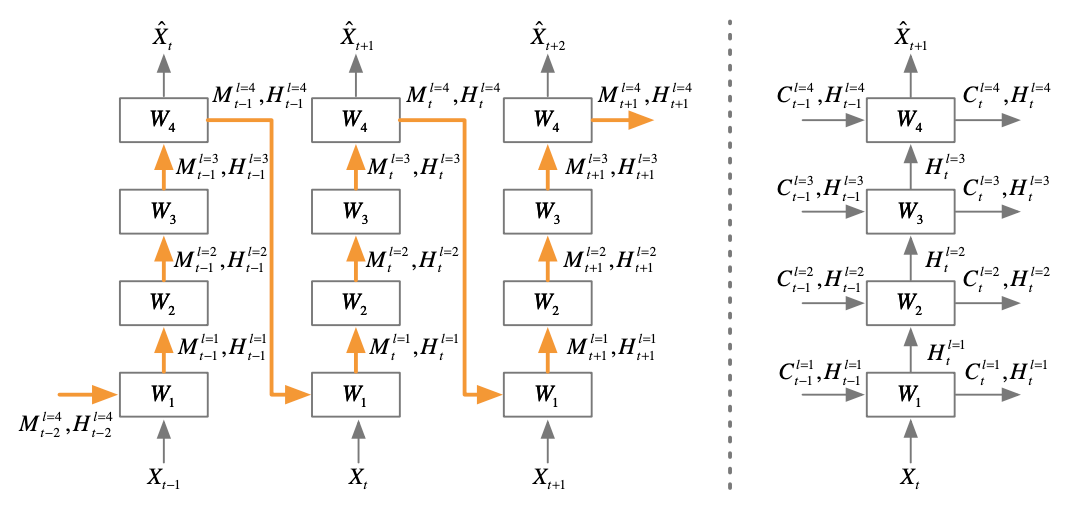
\includegraphics[width=150mm]{figures/predrnn_memory.png}
            \caption{左がPredRNNにおけ時空間メモリフロー、右がConvLSTMのメモリフローである。このような異なるレベルの層を通過するメモリフローにより、多様な抽象度の表現を学習することができる。}
            \label{fig:predrnn}
          \end{center}
        \end{figure}
        
        \subsubsection{時空間LSTMユニット (ST-LSTM)}
          時空間メモリフローは空間情報の効果的な伝達を可能にするが、水平方向(時間方向)のメモリフローを省略すると、時間的一貫性を犠牲にしてしまう。
          PredRNNでは、標準的なLSTMユニットを、時空間メモリセルとゲート構造を導入した時空間LSTM(ST-LSTM)ユニットに置き換える。
          ST-LSTMユニットは、時間メモリセルと時空間メモリセルの両方を維持し、それらを縦方向および横方向に流すことにより、一定の時間一貫性を担保しながら、異なる抽象度レベルでの特徴を捉える。
          また、ST-LSTMは1x1の畳み込み層を使用して次元削減を行い、隠れ状態の次元をメモリセルと同じにする。この構造により、PredRNNは時空間データの複雑なダイナミクスを捉え、より正確な予測を生成することができる。

          時空間LSTMの数学的定式化は以下の通りである。
          ここで、\( \ast \) は畳み込み演算を、\( \circ \) はアダマール積(要素ごとの積)を示す。
          \( W \) と \( b \) は重みとバイアスパラメータ、\( \sigma \) はシグモイド活性化関数、\( \tanh \) は双曲線正接活性化関数を指す。
          \( X_t \) は時刻 \( t \) の入力、\( H_t^l \) は隠れ状態、\( C_t^l \) は標準的なLSTMセル、\( M_t^l \) は時空間メモリセルを表す。
          
          \begin{align}
          g_t &= \tanh(W_{xg} \ast X_t + W_{hg} \ast H_{t-1}^l + b_g) \\
          i_t &= \sigma(W_{xi} \ast X_t + W_{hi} \ast H_{t-1}^l + W_{mi} \circ M_{t-1}^l + b_i) \\
          f_t &= \sigma(W_{xf} \ast X_t + W_{hf} \ast H_{t-1}^l + W_{mf} \circ M_{t-1}^l + b_f) \\
          C_t^l &= f_t \circ C_{t-1}^l + i_t \circ g_t \\
          g_t' &= \tanh(W_{xg}' \ast X_t + W_{mg} \ast M_{t-1}^l + b_g') \\
          i_t' &= \sigma(W_{xi}' \ast X_t + W_{mi} \ast M_{t-1}^l + b_i') \\
          f_t' &= \sigma(W_{xf}' \ast X_t + W_{mf} \ast M_{t-1}^l + b_f') \\
          M_t^l &= f_t' \circ M_{t-1}^l + i_t' \circ g_t' \\
          o_t &= \sigma(W_{xo} \ast X_t + W_{ho} \ast H_{t-1}^l + W_{co} \ast C_t^l + W_{mo} \ast M_t^l + b_o) \\
          H_t^l &= o_t \circ \tanh(W_{1 \times 1} \ast [C_t^l, M_t^l])
          \end{align}
          
          この構造により、PredRNNは時空間データの複雑なダイナミクスを捉え、より正確な未来予測を生成する。
          
          \begin{figure}[htbp]
            \begin{center}
              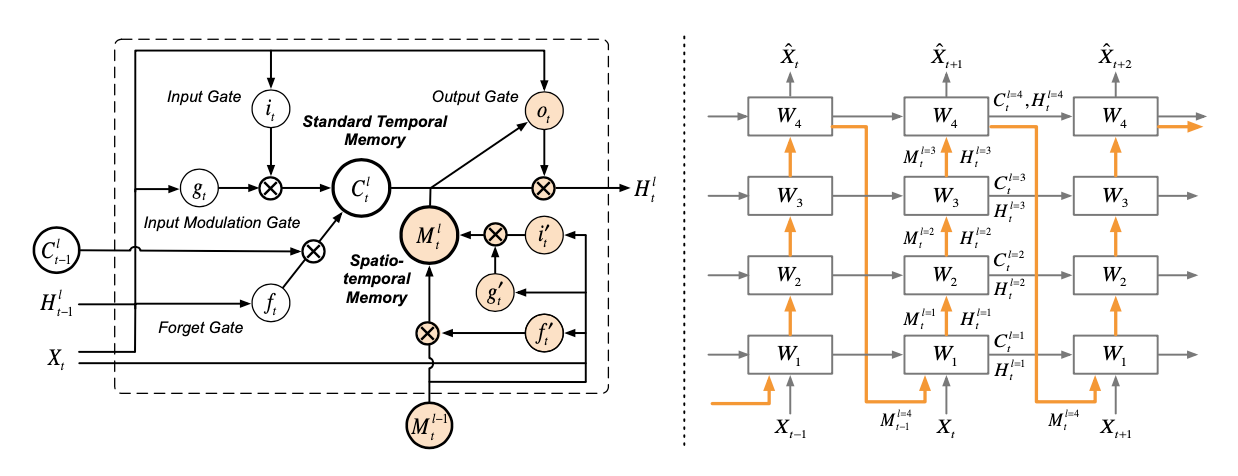
\includegraphics[width=160mm]{figures/predrnn_unit.png}
              \caption{左がST-LSTMユニット、右がPredRNNのメモリフロー。オレンジ色のノードは、従来のConvLSTMと異なるPredRNN独自の構造を示す。PredRNN内のオレンジ色の矢印は、時空間メモリ\( M_t^l \)の移行経路を示す。}
              \label{fig:stlstm}
            \end{center}
          \end{figure}
        
    \subsection{各ゲート}

    \subsection{Motion-Aware Unit(MAU)}
      Motion-Aware Unit (MAU)は、Zheng et al.(2021)によって発表された、フレーム間のダイナミクスをより効率的に捉えるために提案された新しい動画予測アーキテクチャである。
      MAUは、PredRNNと似た積層LSTMの構造を持ち、そのLSTMユニットをMAUセルによって置き換えている。
      MAUセルは、注意(Attention)モジュールと融合(Fusion)モジュールの2つの部分から構成されており、PredRNNにおける時空間LSTMユニットをさらに拡張したものである。
      このような変更により、時間的受容野

      本研究では、このMAUを用いて太陽全球紫外線画像の予測を行う。
      
      \subsubsection{アーキテクチャ}
      動画予測モデルでは、出力中の時間ステップが進むほど、時間情報の不確実性が増加するため、予測誤差が劇的に加速してしまう。この問題を解決するため、動画予測モデルはより幅広い時間ステップから有用な特徴を保存し活用する必要がある。すなわち、時間的受容野を拡張する必要がある。
      このような問題に対するアプローチとして、Yunbo et al. (2019)によって提案された、三次元畳み込みを導入したE3D-LSTMがあったが、非常に高い計算コストを必要とするという課題があった。
      
      \begin{figure}[htbp]
        \begin{center}
          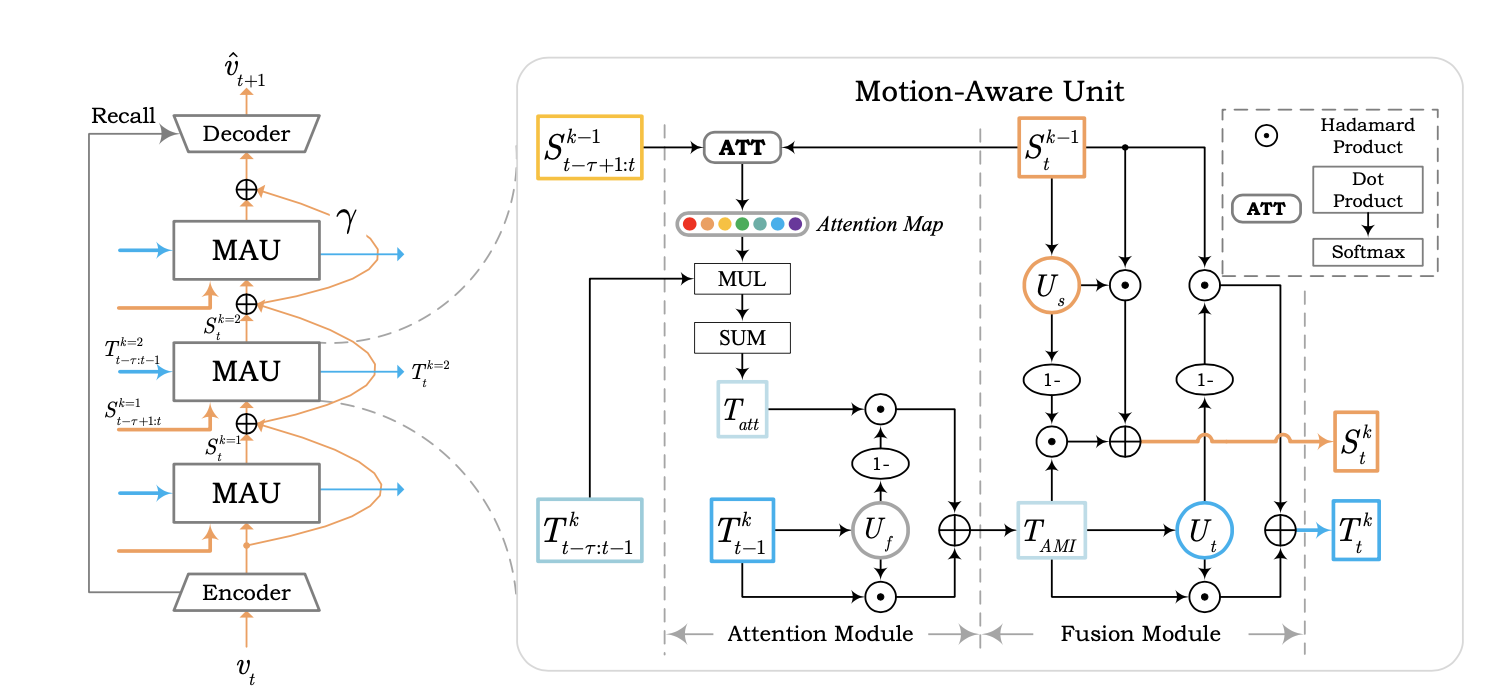
\includegraphics[width=160mm]{figures/mau.png}
          \caption{キャプション}
          \label{fig:mau_attention}
        \end{center}
      \end{figure}
        

      \subsubsection{融合モジュール}
      融合モジュールは、拡張された動きの情報(AMI)と現在の外観情報(現在の空間的状態)を最終的な予測フレームに統合するために使用されます。
          
      \subsubsection{情報リコールスキーム}
      MAUでは、エンコーダとデコーダ間で情報損失を防ぐために、情報リコールスキームが採用されています。これにより、デコーダは多レベルのエンコードされた情報を思い出し、予測の視覚的品質を向上させることができます。    

      \subsubsection{主な実験結果}
      MAUは、複数のデータセットで評価され、その中にはMoving MNIST、KITTI、Caltech Pedestrian、TownCentreXVID、Something-Something V2が含まれる。
      MAUは64の隠れ状態チャンネルを持ち、5×5のカーネルサイズとストライド1の統合畳み込み演算子を使用しています。すべての実験はAdamオプティマイザで最適化され、訓練プロセスを安定させるために各統合畳み込み層の後にレイヤー正規化演算子が使用されています.